% Template for Cogsci submission with R Markdown

% Stuff changed from original Markdown PLOS Template
\documentclass[10pt, letterpaper]{article}

\usepackage{cogsci}
\usepackage{pslatex}
\usepackage{float}
\usepackage{caption}

% amsmath package, useful for mathematical formulas
\usepackage{amsmath}

% amssymb package, useful for mathematical symbols
\usepackage{amssymb}

% hyperref package, useful for hyperlinks
\usepackage{hyperref}

% graphicx package, useful for including eps and pdf graphics
% include graphics with the command \includegraphics
\usepackage{graphicx}

% Sweave(-like)
\usepackage{fancyvrb}
\DefineVerbatimEnvironment{Sinput}{Verbatim}{fontshape=sl}
\DefineVerbatimEnvironment{Soutput}{Verbatim}{}
\DefineVerbatimEnvironment{Scode}{Verbatim}{fontshape=sl}
\newenvironment{Schunk}{}{}
\DefineVerbatimEnvironment{Code}{Verbatim}{}
\DefineVerbatimEnvironment{CodeInput}{Verbatim}{fontshape=sl}
\DefineVerbatimEnvironment{CodeOutput}{Verbatim}{}
\newenvironment{CodeChunk}{}{}

% cite package, to clean up citations in the main text. Do not remove.
\usepackage{apacite}

% KM added 1/4/18 to allow control of blind submission
\cogscifinalcopy

\usepackage{color}

% Use doublespacing - comment out for single spacing
%\usepackage{setspace}
%\doublespacing


% % Text layout
% \topmargin 0.0cm
% \oddsidemargin 0.5cm
% \evensidemargin 0.5cm
% \textwidth 16cm
% \textheight 21cm

\title{The latent factor structure of developmental change in early childhood}

\usepackage{amsmath}
\usepackage{bm}
\usepackage{xcolor}
\newcommand\myworries[1]{\textcolor{red}{#1}}
\usepackage{booktabs}
\usepackage{longtable}
\usepackage{array}
\usepackage{multirow}
\usepackage{wrapfig}
\usepackage{float}
\usepackage{colortbl}
\usepackage{pdflscape}
\usepackage{tabu}
\usepackage{threeparttable}
\usepackage{threeparttablex}
\usepackage[normalem]{ulem}
\usepackage{makecell}
\usepackage{xcolor}

\author{Anonymous Cogsci Submission}

\begin{document}

\maketitle

\begin{abstract}
Piaget proposed that development proceeded in stages; more recently
researchers have proposed modular theories in which different abilities
develop on their own timetable. Despite the abundance of theory, there
is little empirical work on the structure of developmental changes in
early childhood. We investigate this question using a large dataset of
parent-reported developmental milestones. We compare a variety of
factor-analytic item response theory models and find that variation in
development from birth to 55 months of age is best described by a model
with three distinct dimensions. We also find evidence that
dimensionality increases across age, with the youngest children
described by a two-factor model. These results provide a model-based
method for linking holistic descriptions of early development to basic
theoretical questions about the nature of change in childhood.

\textbf{Keywords:}
child development; milestones; item response theory; model comparison
\end{abstract}

\hypertarget{introduction}{%
\section{Introduction}\label{introduction}}

How do young children grow and change? Is child development a single
unified process or a host of different processes, each with their own
constraints and timescale? Piaget famously proposed a stage theory in
which many seemingly distinct mental processes developed in concert
through the operation of the same principles across domains (Flavell,
1963). In contrast, modern theories propose that different facets of
children's mental life develop on their own timetable (Gelman \& Meck,
1983). And the grandmother of one author of this paper was known to
assert that developmental milestones were in compensatory relationships
with one another (``children either walk early or else they talk
early'').

This question is important not only from a theoretical perspective but
also for application. The process of assessing children's developmental
status critically depends on our assumptions about the nature of that
status --- in particular, whether there is a single unified process that
can be measured via some score derived from subprocesses. In this sense,
questions about the nature and structure of development are psychometric
questions (Borsboom, 2005). Such psychometric analysis investigating the
dimensionality of change has been studied extensively in the case of
cognitive aging (e.g., Balinsky, 1941; Li, Nuttall, \& Zhao, 1999) but
has received less attention in early childhood.

Our goal is to describe the psychometric structure of development. We
take as our starting point the idea that psychometric models can
instantiate hypotheses about psychological structure in ways that can be
assessed via their fit to data. We adopt the framework of item response
theory (IRT). IRT models allow us to capture how responses to such
questions track both with individual children's abilities as well as
with the measurement properties of the questions (and underlying
milestones). In particular, our interest is in comparing within a family
of multidimensional IRT models in order to gain insight into the
underlying dimensionality of early childhood development.

In a standard factor-analytic approach (which multi-dimensional IRT
extends), a solution with N factors partitions observed variance into
factors, suggesting dimensions of variation in the sample. One
substantial complication to this perspective for analyzing developmental
data is the issue that the dimensionality of children's variation could
itself change developmentally. Indeed, the dedifferentiation hypothesis
of cognitive aging --- that distinct factors collapse --- is such a
hypothesis (Frias, Lövdén, Lindenberger, \& Nilsson, 2007). To address
this challenge, we use a new set of cross-validation methods to
investigate changes in dimensionality.

We use milestone data for our investigation. Global assessment of
developmental status via a series of binary questions (e.g., ``Can your
child walk at least ten steps unassisted?'') is both a standard feature
of pediatrician visits (Sheldrick et al., 2019) and a gold standard for
child development in the research and intervention communities (Bayley,
2009; Bricker et al., 1999; McCoy, Gonzalez, \& Jones, 2019). In such
assessments, which are typically but not always conducted via parent
report, developmental progress is pooled across domains like motor
development or language. Thus, these instruments implicitly assume a
unifactorial model, although some also provide subscale scores (Bayley,
2009).

Unfortunately, these instruments are commercial products, and hence
normative data at the item level are typically not available for
analysis. In the current paper, we thus analyze a new set of data from a
set of 414 milestone questions administered online to a group of 1946
middle-class Mexican parents of children from 0 to 55 months of age.
This very comprehensive milestone set allows us to ask questions about
how variation in developmental growth can be partitioned across age and
face-valid domains (language, cognition, motor, and socio-emotional
development).

We first describe our dataset. We then introduce the family of item
response models that we use and the way in which we compare performance
across these models. These models allow us to consider the overall
dimensionality of our dataset, which we then follow up on by looking for
evidence of change in dimensionality across development. We end by
considering the limitations, implications, and next steps for this work.

\hypertarget{data}{%
\section{Data}\label{data}}

A child's development can be thought of as the set of developmental
milestones that they have reached at a particular point in time. This
conceptualization results in data with the same structure as the item
response data common to educational measurement. In education, item
response data is most typically students responding to test items (i.e.,
questions) and, in the dichotomous case, getting each question either
correct or incorrect. In the context of child development, the child is
the ``student,'' and each developmental milestone is the ``item.''

Data were provided by Kinedu, Inc., a developer of parenting
applications. We consider the 1946 children between 2 and 55 months of
age whose parents responded to all 414 of the developmental milestones.
Kinedu, Inc.~mapped each milestone to a face-valid group: physical,
cognitive, linguistic, or social \& emotional. Table \ref{tab:examples}
shows the number of developmental milestones in each group along with an
example milestone from each group translated to English.

\begin{CodeChunk}
\begin{table}[!h]

\caption{\label{tab:examples}Developmental milestone groups and examples}
\centering
\fontsize{8}{10}\selectfont
\begin{tabular}[t]{l|r|l}
\hline
Group & Milestones & Example milestone\\
\hline
Physical & 180 & Stands on their toes\\
\hline
Cognitive & 100 & Finds objects on the floor\\
\hline
Linguistic & 75 & Babbles to imitate conversations\\
\hline
Social \& Emotional & 59 & Complains when play is stopped\\
\hline
\end{tabular}
\end{table}

\end{CodeChunk}

Figure \ref{fig:growth} shows the age (in months) and number of
completed milestones for each child. At 12 months old, most children
have reached about 200 developmental milestones. At 24 months old, most
children have reached about 300 developmental milestones. At 48 months
old, most children have reached about 375 of the 414 developmental
milestones.

\begin{CodeChunk}
\begin{figure}[tb]
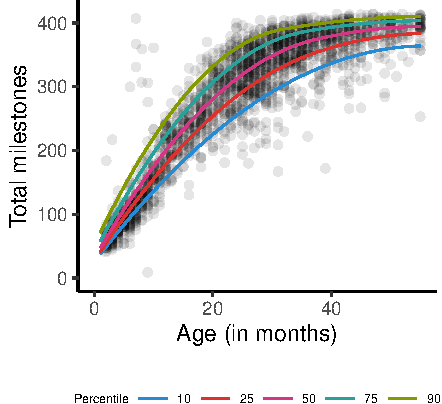
\includegraphics{figs/growth-1} \caption[Number of milestones by age and percentile curves]{Number of milestones by age and percentile curves. Dots represent individual children. }\label{fig:growth}
\end{figure}
\end{CodeChunk}

\hypertarget{methods}{%
\section{Methods}\label{methods}}

We frame the assessment of the dimensionality of child development as a
model comparison question.

\hypertarget{models}{%
\subsection{Models}\label{models}}

Item response theory offers a suite of models with which to model item
response data. We adopt the notation used in Chalmers \& al. (2012). Let
\(i = 1, \ldots, I\) represent the distinct children and
\(j = 1, \ldots, J\) the developmental milestones. The item response
data is stored in a matrix, \(y\), where element \(y_{ij}\) denotes if
the \(i\)th child has or has not achieved the \(j\)th developmental
milestone as reported by their parent/guardian. Each model represents
the \(i\)th child's development using \(m\) latent factors
\(\boldsymbol{\theta}_{i}=(\theta_1, \dots, \theta_m)\). The \(j\)th
milestone's discriminations (i.e.~slopes)
\(\boldsymbol{a_j}=(a_1, \dots, a_m)\) capture the latent factor
loadings onto that milestone.

We fit five two-parameter logistic (2PL) models where a child's
development is represented by \(m = 1, \ m = 2, \ m = 3, \ m = 4\) and
\(m = 5\) latent factors. Hereafter, we, for example, refer to a 2PL
model with \(m = 4\) latent factors as a 4F 2PL model. According to the
2PL model, the probability of a child having achieved a developmental
milestone is \[
P(y_{ij} = 1 | \boldsymbol{\theta_i}, \boldsymbol{a_j}, b_j) = \sigma(\boldsymbol{a}_{j}^{\top}\boldsymbol{\theta_i} + b_j)
\] where \(b_j\) is the milestone easiness (i.e.~intercept) and
\(\sigma(x) = \frac{e^x}{e^x + 1}\) is the standard logistic function.
As an example, Figure \ref{fig:icc} shows item characteristic curves
from the 1F 2PL model for the items in Table \ref{tab:examples}. Item
characteristic curves show how \(P(y_{ij} = 1)\) changes as \(\theta_i\)
changes for a particular item. These curves reveal that babbling is
unrelated to development. On the other hand, finding objects on the
floor is highly related to development with most children with
\(\theta_i\) greater than -1.5 having reached this milestone.

We explored 3PL models, which add a guessing parameter to the 2PL model,
but they did not fit better and so we omit them for space, preferring
instead to look at the more interesting factor structure. We do include
a 1F Rasch model where all of the discriminations,
\(\boldsymbol{a}_{j}\), are set to 1 for each item.

Each of these models learn the latent factor structure entirely from the
data, making them exploratory. The bifactor model offers an alternative
specification where each milestone loads onto a general factor
\(\theta_0\) and a specific factor \(\theta_s\) (Cai, Yang, \& Hansen,
2011). The assignment of each developmental milestone to its specific
factor is an opportunity to specify the latent factor structure, making
the model confirmatory as opposed to exploratory. We map each milestone
to its specific factor according to the four developmental milestone
groups shown in Table \ref{tab:examples}. For the bifactor model, the
probability of a child having achieved a developmental milestone is \[
P(y_{ij} = 1 | \theta_0, \theta_s, a_0, a_s) = \sigma(a_0\theta_0 + a_s\theta_s + b_j).
\]

Computing is done in R (R Core Team, 2019), model fitting in the R
package mirt (Chalmers \& al., 2012), and data wrangling/visualization
in the set of R packages known as the tidyverse (Wickham, 2017).

\begin{CodeChunk}
\begin{figure}[tb]
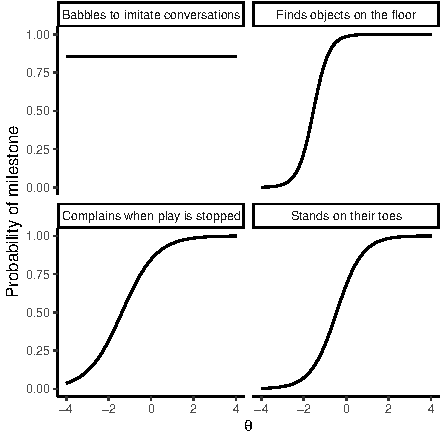
\includegraphics{figs/icc-1} \caption[Example item characteristic curves]{Example item characteristic curves. Babbling is unrelated to a child's development whereas finding objects on the floor is highly related to development.}\label{fig:icc}
\end{figure}
\end{CodeChunk}

\hypertarget{modelcompare}{%
\subsection{Model comparison}\label{modelcompare}}

Model comparison in IRT typically uses information criterion such as AIC
and BIC (Maydeu-Olivares, 2013). However, these methods are not
guaranteed to work with modest sample sizes or misspecification
(McDonald \& Mok, 1995). Instead, we use a marginalized version of
cross-validation. In essence, we partition the data into folds based on
the children (i.e.~the rows of the item response matrix). Then for each
fold, we estimate the item parameters using all but that fold, and
calculate the likelihood of that fold by integrating over \(g(\theta)\).

Mathematically and following notation similar to Vehtari, Gelman, \&
Gabry (2017), we partition the data into \(K\) subsets \(y^{(k)}\) for
\(k = 1, \dots, K\). Each model is fit separately to each training set
\(y^{(-k)}\) yielding item parameter estimates which we compactly denote
\(\Psi_j^{(-k)}\). The predictive (i.e.~out-of-sample or
cross-validated) likelihood of \(y^{(k)}\) is

\[
p(y^{(k)} | y^{(-k)}) = \prod_{i \in i^{(k)}}^{I} \int_\theta \prod_{j=1}^{J} \hat{\text{Pr}}(y_{ij}^{(k)} | \Psi_j^{(-k)}, \theta) g(\theta)d\theta.
\]

The ultimate quantity of interest for each model is the log predictive
likelihood for the entire item response matrix, which is defined as

\[
\text{lpl } y = \sum_{k = 1}^{K} \log p(y^{(k)} | y^{(-k)}).
\]

\hypertarget{results}{%
\section{Results}\label{results}}

Table \ref{tab:results} shows the number of parameters, the in-sample
log likelihood (which neccessarily increases with more parameters), and
the \(\text{lpl } y\) defined in the
\protect\hyperlink{modelcompare}{model comparison section}. The 3F 2PL
model performs best which is evidence that child development between the
ages of 2 and 55 months follows a multidimensional path.

\begin{CodeChunk}
\begin{table}[!h]

\caption{\label{tab:results}Model performance: The 3F 2PL performs best as measured by lpl y}
\centering
\fontsize{8}{10}\selectfont
\begin{tabular}[t]{l|r|r|r}
\hline
model & parameters & log-likelihood (in-sample) & lpl y (out-of-sample)\\
\hline
1F Rasch & 415 & -254983.9 & -255441.5\\
\hline
1F 2PL & 828 & -222072.9 & -223105.6\\
\hline
2F 2PL & 1241 & -212896.4 & -214491.4\\
\hline
Bifactor & 1242 & -210030.2 & -211682.2\\
\hline
*3F 2PL* & 1653 & -208806.0 & -210960.5\\
\hline
4F 2PL & 2064 & -208113.9 & -211022.8\\
\hline
5F 2PL & 2474 & -207316.2 & -211036.3\\
\hline
\end{tabular}
\end{table}

\end{CodeChunk}

\hypertarget{understanding-the-latent-factor-structure}{%
\subsection{Understanding the latent factor
structure}\label{understanding-the-latent-factor-structure}}

To understand each of the three factors in the best performing model, we
fit the model to the the full dataset. We then estimate the factor
loadings (i.e.~discriminations or slopes) using a varimax rotation. The
varimax rotation results in orthogonal and, therefore, more
interpretable factors (Kaiser, 1959). Figure \ref{fig:factorloadings}
shows the distribution of factor loadings for each group on each of the
three factors. The first factor loads mainly on cognitive and linguistic
milestones. The second factor is a combination of each of the groups
with the strongest loadings on the physical and social \& emotional
milestones. The third mainly load positively on linguistic milestones
and, interestingly, negatively on physical milestones.

\begin{CodeChunk}
\begin{figure}[tb]
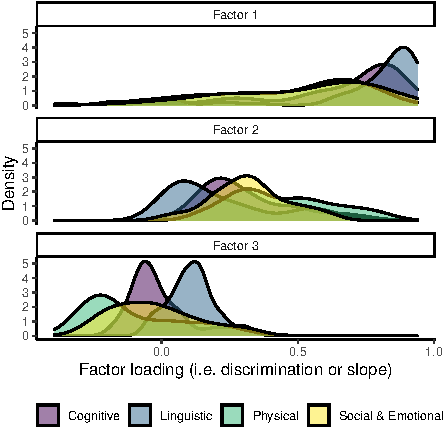
\includegraphics{figs/factorloadings-1} \caption[Factor loadings by group]{Factor loadings by group}\label{fig:factorloadings}
\end{figure}
\end{CodeChunk}

We also estimate the factor scores for each child using expected a
posteriori (EAP) with a three dimensional standard normal distribution
(Embretson \& Reise, 2013). Figure \ref{fig:factorscores} shows the
relationship between age and factor score for each factor. The first
factor, perhaps unsurprisingly, has a high correlation (r = 0.9) with
age. The second factor has a strong association with age from 2 to 16
months but thereafter is unrelated to age. By and large, the third
factor does not have any association with age.

\begin{CodeChunk}
\begin{figure}[tb]
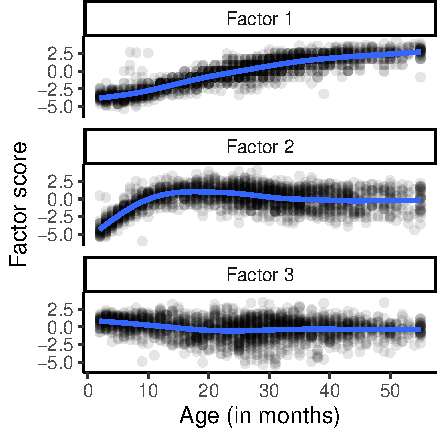
\includegraphics{figs/factorscores-1} \caption[The first factor is highly associated with age]{The first factor is highly associated with age}\label{fig:factorscores}
\end{figure}
\end{CodeChunk}

\hypertarget{dimensionality-across-the-age-span}{%
\subsection{Dimensionality across the
age-span}\label{dimensionality-across-the-age-span}}

For the entire dataset, we've shown evidence that the 2PL model with
3-factors performs best. But is this latent factor dimensionality
consistent across age-span? For example, perhaps for very young children
1-factor is sufficient and then later on 2- and then 3-factors become
valuable. We take two approaches to assessing the dimensionality of
child development across the age-span. First, we examine the performance
of each of the models by age. Second, we partition the data by age and
use the same cross-validation procedure to find the best fitting model
in each partition.

\hypertarget{full}{%
\subsection{Full model}\label{full}}

Figure \ref{fig:byage} displays the mean cross-validated log likelihood
for each model by age, which comes from the k-fold cross-validation
described in the \protect\hyperlink{modelcompare}{model comparison}
section. For each student, we calculate the marginalized out-of-sample
likelihood based on the item parameters \(\Psi_j^{(-k)}\) from fitting
the model to \(y^{(-k)}\), the folds of data that do not include the
student. As a reminder, students are assigned to folds randomly and not
by age.

Figure \ref{fig:byage} shows how both the 3F 2PL and bifactor models
compare to the 2F 2PL model in terms of cross-validated log likelihood
for each age. The 2F 2PL outperforms both models for children younger
than 7 months old. For children older than 11 months old, both the 3F
2PL and bifactor models outperform the 2F 2PL model with the 3F 2PL
model tending to perform best.

\begin{CodeChunk}
\begin{figure}[tb]
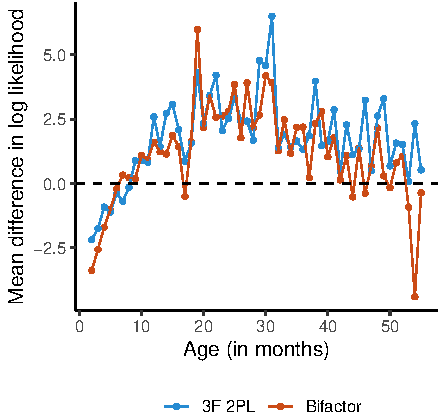
\includegraphics{figs/byage-1} \caption[Comparing the 4F 2PL and Bifactor models to the 2F 2PL]{Comparing the 4F 2PL and Bifactor models to the 2F 2PL}\label{fig:byage}
\end{figure}
\end{CodeChunk}

\hypertarget{age-partitioned-models}{%
\subsection{Age-partitioned models}\label{age-partitioned-models}}

As another method of examining the dimensionality of child development
across the age span, we create four partitions of the data based on the
ages of the children. We then cross-validate the 2PL models
independently in each partition. This allows us to examine the
dimensionality for each age group separately. For each age partition, we
drop milestones where less than 2.5\% or greater than 97.5\% of children
have reached the milestone. We drop these milestones because they
contain little information and make the models less stable. This process
results in, for example, 432 children and 359 milestones in the 13-24
month old partition.

Figure \ref{fig:partage} shows the results of this analysis. Consistent
with our findings in the \protect\hyperlink{full}{previous section}, the
best fitting model contains a lower dimensional factor structure for
younger children. The best fitting model is the 2F 2PL for the partition
of data containing children two to 12 months old, whereas the best
fitting model is the 3F 2PL for the partitions containing older
children.

\begin{CodeChunk}
\begin{figure}[tb]
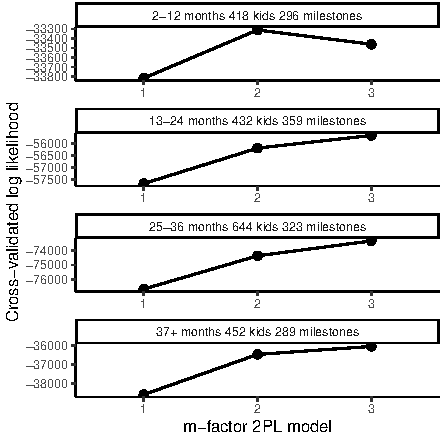
\includegraphics{figs/partage-1} \caption[2F 2PL best for young kids]{2F 2PL best for young kids; 3F 2PL best for older kids}\label{fig:partage}
\end{figure}
\end{CodeChunk}

\hypertarget{discussion}{%
\section{Discussion}\label{discussion}}

Is child development a single unified process or a host of different
processes? Stage theories assume synchronization in developmental
changes across distinct domains like language, social/emotional
development, and cognition. In contrast, more modern modular theories
tend to assume that particular aspects of development proceed ``on their
own schedule'' (Spelke, Breinlinger, Macomber, \& Jacobson, 1992). Here,
inspired by psychometric studies of age-related changes in cognition, we
explored this issue in a large dataset of children's developmental
milestones. Our premise was that understanding the nature of variation
in milestones could help shed light on whether children's developmental
change covaries across domains within a single factor or whether it is
split into multiple factors.

Using multi-factor item response theory models and a new
cross-validation method for model comparison, we found that a
three-factor model best described developmental variation across the
first 55 months. While the first factor described a large amount of
shared variation in development, the structure of these factors did
suggest some differentiation between cognitive/linguistic development,
physical development, and socio/emotional development. Further, we found
that the dimensionality of variation increased developmentally: 2--12
month-olds were best described by a two-dimensional model, while older
groups were best described by a three-dimensional model. This analysis
provides tentative support for a developmental differentiation
hypothesis, where different domains of development vary across
individuals in a way that is increasingly more independent over age.

Our study has a number of limitations that should inform future work.
Our dataset is cross-sectional, meaning that we are only describing
variation across individuals rather than the coherence of factors within
individuals. Second, we relied on parent report, which can have
significant biases and limitations, especially in its precision
regarding capacities that are difficult to observe (e.g., cognitive
abilities; Feldman et al., 2000; Frank, Braginsky, Marchman, \&
Yurovsky, 2020). Third, our data come from a very specific population
group (middle- and upper-class Mexican parents whose children were in
group care) and hence caution is warranted in generalizing to other
populations.

This work has significant practical implications: Measures of
developmental change should not assume that a single score captures all
of the variance in developmental change. Thus, understanding the
generality of our conclusions is an important practical goal that could
affect the structure of a variety of standardized developmental
inventories in broad clinical and research use.

The nature of developmental variation is of core importance to our
theorizing about the mechanisms of child development. Yet this variation
has often been assumed to be unifactorial or multifactorial without
formal evaluation. Our work here takes a first step towards using
psychometric models to evaluate this dimensionality empirically.

\hypertarget{acknowledgements}{%
\section{Acknowledgements}\label{acknowledgements}}

{[}BLINDED{]}

\hypertarget{references}{%
\section{References}\label{references}}

\setlength{\parindent}{-0.1in} 
\setlength{\leftskip}{0.125in}

\noindent

\hypertarget{refs}{}
\leavevmode\hypertarget{ref-balinsky1941analysis}{}%
Balinsky, B. (1941). An analysis of the mental factors of various age
groups from nine to sixty. \emph{Genetic Psychology Monographs}.

\leavevmode\hypertarget{ref-bayley2009bayley}{}%
Bayley, N. (2009). \emph{Bayley-iii: Bayley scales of infant and toddler
development}. Giunti OS.

\leavevmode\hypertarget{ref-borsboom2005measuring}{}%
Borsboom, D. (2005). \emph{Measuring the mind: Conceptual issues in
contemporary psychometrics}. Cambridge University Press.

\leavevmode\hypertarget{ref-bricker1999ages}{}%
Bricker, D., Squires, J., Mounts, L., Potter, L., Nickel, R., Twombly,
E., \& Farrell, J. (1999). Ages and stages questionnaire. \emph{Paul H.
Brookes: Baltimore}.

\leavevmode\hypertarget{ref-cai2011generalized}{}%
Cai, L., Yang, J. S., \& Hansen, M. (2011). Generalized full-information
item bifactor analysis. \emph{Psychological Methods}, \emph{16}(3), 221.

\leavevmode\hypertarget{ref-chalmers2012mirt}{}%
Chalmers, R. P., \& al. (2012). Mirt: A multidimensional item response
theory package for the r environment. \emph{Journal of Statistical
Software}, \emph{48}(6), 1--29.

\leavevmode\hypertarget{ref-embretson2013item}{}%
Embretson, S. E., \& Reise, S. P. (2013). \emph{Item response theory}.
Psychology Press.

\leavevmode\hypertarget{ref-feldman2000measurement}{}%
Feldman, H. M., Dollaghan, C. A., Campbell, T. F., Kurs-Lasky, M.,
Janosky, J. E., \& Paradise, J. L. (2000). Measurement properties of the
macarthur communicative development inventories at ages one and two
years. \emph{Child Development}, \emph{71}(2), 310--322.

\leavevmode\hypertarget{ref-flavell1963developmental}{}%
Flavell, J. H. (1963). The developmental psychology of jean piaget.

\leavevmode\hypertarget{ref-wordbank}{}%
Frank, M., Braginsky, M., Marchman, V., \& Yurovsky, D. (2020).
Variability and consistency in early language learning. \emph{Child
Development}.

\leavevmode\hypertarget{ref-de2007revisiting}{}%
Frias, C. M. de, Lövdén, M., Lindenberger, U., \& Nilsson, L.-G. (2007).
Revisiting the dedifferentiation hypothesis with longitudinal
multi-cohort data. \emph{Intelligence}, \emph{35}(4), 381--392.

\leavevmode\hypertarget{ref-gelman1983preschoolers}{}%
Gelman, R., \& Meck, E. (1983). Preschoolers' counting: Principles
before skill. \emph{Cognition}, \emph{13}(3), 343--359.

\leavevmode\hypertarget{ref-kaiser1959computer}{}%
Kaiser, H. F. (1959). Computer program for varimax rotation in factor
analysis. \emph{Educational and Psychological Measurement},
\emph{19}(3), 413--420.

\leavevmode\hypertarget{ref-li1999test}{}%
Li, C., Nuttall, R. L., \& Zhao, S. (1999). A test of the piagetian
water-level task with chinese students. \emph{The Journal of Genetic
Psychology}, \emph{160}(3), 369--380.

\leavevmode\hypertarget{ref-maydeu2013goodness}{}%
Maydeu-Olivares, A. (2013). Goodness-of-fit assessment of item response
theory models. \emph{Measurement: Interdisciplinary Research and
Perspectives}, \emph{11}(3), 71--101.

\leavevmode\hypertarget{ref-mccoy2019preschool}{}%
McCoy, D. C., Gonzalez, K., \& Jones, S. (2019). Preschool
self-regulation and preacademic skills as mediators of the long-term
impacts of an early intervention. \emph{Child Development},
\emph{90}(5), 1544--1558.

\leavevmode\hypertarget{ref-mcdonald1995goodness}{}%
McDonald, R. P., \& Mok, M. M.-C. (1995). Goodness of fit in item
response models. \emph{Multivariate Behavioral Research}, \emph{30}(1),
23--40.

\leavevmode\hypertarget{ref-rcore}{}%
R Core Team. (2019). \emph{R: A language and environment for statistical
computing}. Vienna, Austria: R Foundation for Statistical Computing.
Retrieved from \url{https://www.R-project.org/}

\leavevmode\hypertarget{ref-sheldrick2019establishing}{}%
Sheldrick, R. C., Schlichting, L. E., Berger, B., Clyne, A., Ni, P.,
Perrin, E. C., \& Vivier, P. M. (2019). Establishing new norms for
developmental milestones. \emph{Pediatrics}, \emph{144}(6).

\leavevmode\hypertarget{ref-spelke1992origins}{}%
Spelke, E. S., Breinlinger, K., Macomber, J., \& Jacobson, K. (1992).
Origins of knowledge. \emph{Psychological Review}, \emph{99}(4), 605.

\leavevmode\hypertarget{ref-vehtari2017practical}{}%
Vehtari, A., Gelman, A., \& Gabry, J. (2017). Practical bayesian model
evaluation using leave-one-out cross-validation and waic.
\emph{Statistics and Computing}, \emph{27}(5), 1413--1432.

\leavevmode\hypertarget{ref-tidy}{}%
Wickham, H. (2017). \emph{Tidyverse: Easily install and load the
'tidyverse'}. Retrieved from
\url{https://CRAN.R-project.org/package=tidyverse}

\bibliographystyle{apacite}


\end{document}
